%!TEX root = ../main.tex
% %

\chapter{Implementation}

\section{Data Preparation}
Once the 20 images comprising the project dataset were split into patches, the dot-annotated set was reannotated using LabelImg. The unannotated patches were then split into train, test, and validation subdirectories in the \verb`/image` directory, and the label files produced from annotation were placed into the corresponding subdirectories in the \verb`/labels` directory (see Figure \ref{directories}). Since Google Colab was being used for computation, the dataset was uploaded to Google Drive to ensure it was easily accessible \& safely stored in the cloud.

\begin{figure}[h!]
	\centering
	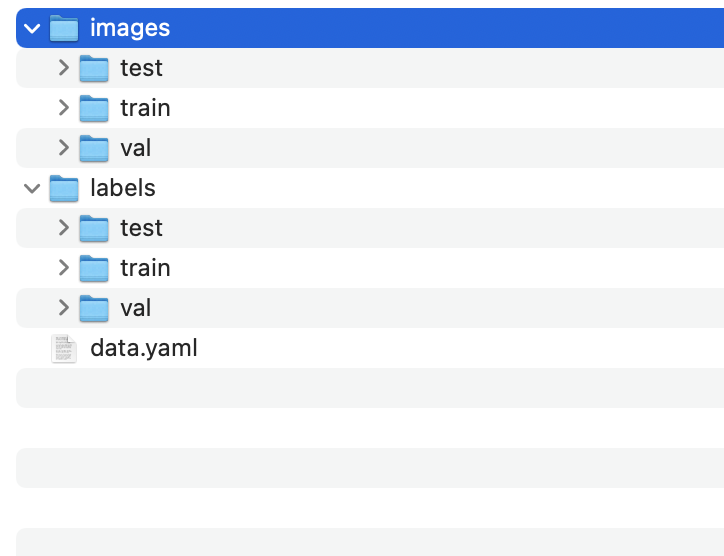
\includegraphics[width=0.5\textwidth]{images/04Implementation/directories.png}
	\caption{Directory structure for the project dataset}
	\label{directories}
\end{figure}

\subsection{Annotation}
The images in Micropics are sparse; cells appear in close groups rather than being evenly distributed. This means that many image patches could be skipped during annotation because they were were empty of cells. The final training set (70\% of the full dataset) comprised 384 images, but only 202 corresponding label files existed after annotation (Version 3), meaning that around 53\% of the training set was comprised of blank patches. The first version of the annotations took around 3 hours to complete.

\section{Training}
Prior to training, Weights and Biases was initialised to collect training statistics. 7 experiments were run; the configurations for each experiment are detailed in Table \ref{configs}.

\subsection{Annotation Revisions}
Disappointing initial results prompted the revision of the data annotations. The model appeared to fail to detect cells and undercounted significantly as a result, so it was decided that the criteria for labelling should be broadened to provide more information for the model to learn from. The annotations were subject to two revisions, both of which took substantially less time than the first attempt. In both revisions, the rules adhered to in the first version were modified:\\

\paragraph{Version 2} included cells which were dot-annotated and unoccluded, but out-of-focus \emph{or} exceeding the edge of the patch (but not both).\\

\paragraph{Version 3,} in addition to the cells included by Version 2's criteria, included those which were both out-of-focus \emph{and} exceeding the edge of the patch edge, and an attempt was made to include occluded cells where they could be told apart.\\
 
\subsection{Train/Test Split}
For the first and second experiments, 50\% of the dataset was reserved for training, with the other 50\% itself being split 50/50 into test and validation sets. After the 2nd run this 50/25/25 split was revised to 70/15/15 to explore the effect of a larger training set.\\

\subsection{Base Model}
In later experiments, the base model was changed from the lightweight and fast YOLOv5s to the more substantial YOLOv5l, an 89MB model with more than 40 million parameters which took more than twice as long to train as YOLOv5s.

\subsection{Epochs}
For the first experiment, a tentative 30 epochs was used to avoid overfitting. It was found in later experiments that increasing the number of epochs did not cause the model to overfit, even at 300 epochs, and that increasing the number of epochs had a pronounced effect on the model's counting capabilities.

\subsection{Batch Size}
Batch size started at 16 and was briefly kept at 32, on the recommendation of \cite{DBLP:journals/corr/abs-1804-07612} to use small batch sizes. However, later experiments instead heeded the recommendation of the YOLOv5 documentation\footnote{Tips for Best Training Results · ultralytics/yolov5 Wiki. (no date). Available at: https://github.com/ultralytics/yolov5/wiki/Tips-for-Best-Training-Results (Accessed: 05/05/2022).} to use substantially higher batch sizes, and this was increased to 128.

\begin{table}
\centering
\begin{tabular}{ |l||l|l|l|l|l|}
\hline
\multicolumn{6}{|c|}{Experiment Configurations} \\
\hline
Experiment & Annotations & Train/Test/Val Split & Batch Size & Epochs & Base Model\\
\hline
1 & v1 & 50/25/25 & 16 & 32 & YOLOv5s\\ 
 2 & v2 & 50/25/25 & 32 & 25 & YOLOv5s\\
 3 & v3 & 70/15/15 & 32 & 25 & YOLOv5s\\
 4 & v3 & 70/15/15 & 32 & 50 & YOLOv5s\\
 5 & v3 & 70/15/15 & 32 & 50 & YOLOv5l\\
 6 & v3 & 70/15/15 & 128 & 300 & YOLOv5s\\ 
 7 & v3 & 70/15/15 & 128 & 300 & YOLOv5l\\
\hline
\end{tabular}
\caption{Configurations for each run of training}
\label{configs}
\end{table}

\section{Counting}
Once the custom detection model is trained and⁠—in principle⁠—capable of detecting all cells in an input image, the detected cells can be counted easily, and the artifact's counting component was developed for this purpose. This component's principal function is \verb|count(directory, edge)|. This function uses YOLOv5's \verb|detect.py| script to run batch inference on all image patches in the \verb`directory` passed. Batch inference returns a \verb|Detections| object which contains a number of Pandas DataFrames, each of which corresponds to an image patch. Each DataFrame includes a row for every object detected in the patch; this allows for easy counting by looping through all the DataFrames, calling \verb|len()| on each to return a count of objects detected in the patch, and summing all patch counts. For the purposes of debugging and qualitative evaluation, \verb|count(...)| also prints the first DataFrame in the \verb|Detections| object, alongside the associated image patch with predicted bounding boxes.\\

It was recognised early on during testing that the model tended to count the same cells twice where they spanned 2 patches, and the fact that inference data was returned in the form of DataFrames allowed for a method to control for this. Since each row in the DataFrame includes the minimum and maximum extents of each predicted bounding box, a condition was included in \verb|count(...)| to simply discard any object with a bounding box that intersects with the top-left edge of the patch (by default, within 2 pixels of the edge, but a value for \verb`edge` can be passed to \verb`count(...)`). This 'trimming' was not applied to the bottom-right edge; the effect of this was that any cell straddling the bottom-right edge of a patch was counted once in that patch, but not counted again if seen in a subsequent one.\\

All patch counts are summed and returned by \verb|count(...)| to provide the count for the full-resolution image. The 4 images in the test set were used to test the model's counting capabilities. The image patches, rather than the full-resolution images, were used for this purpose: YOLOv5's documentation states that for best results, the size of the images on which inference is run should be the same as that of the training images\footnote{Tips for Best Training Results · ultralytics/yolov5 Wiki. (no date). Available at: https://github.com/ultralytics/yolov5/wiki/Tips-for-Best-Training-Results (Accessed: 05/05/2022).}.\\

\begin{lstlisting}[language=Python, caption={The counting component's principal function, count(...)}, label={def_count}]
def count(img: StringType, edge: int = 2):
  patches = []

  # Run inference on all patches in the image directory
  for i in os.listdir(f'/content/drive/MyDrive/CM4105/dataset/images/{img}'):
    patches.append(f'/content/drive/MyDrive/CM4105/dataset/images/{img}/' + i)
  results = model(patches)

  # Iterate through the DataFrames and sum their lengths for a count of cells in the image
  dfs = results.pandas().xyxy
  count = 0
  for df in dfs:
    # Remove cells along the top-left edges of the image
    df_trim = df.loc[df['xmin'] > edge]
    df_trim = df_trim.loc[df['ymin'] > edge]
    count += len(df_trim)

  # Print the first DataFrame in the results
  print(f'First patch of image {img}:')
  display(dfs[0])

  # Display the first image in the results
  results.render()
  cv2_imshow(results.imgs[0])

  return count
\end{lstlisting}

\begin{figure}[h!]
	\centering
	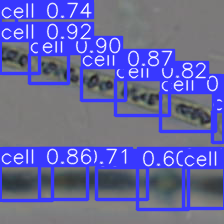
\includegraphics[width=0.5\textwidth]{images/04Implementation/patch.png}
	\caption{Predictions by custom YOLOv5 model on a patch from the test set (image)}
\end{figure}

% \begin{table}
% \centering
% \begin{tabular}{ |l||l|l|l|l|l|l|}
% \hline
% \multicolumn{7}{|c|}{Model Predictions} \\
% \hline
% xmin &        ymin &        xmax &        ymax &  confidence &  class &  name \\
% \hline
% 183.162689 &  167.604874 &  224.000000 &  208.682205 &    0.927962 &      0 &  cell \\
% 0.000000 &   40.554379 &   39.667694 &   73.713120 &    0.924108 &      0 &  cell \\
% 29.663275 &   54.058395 &   68.274818 &   83.056252 &    0.903497 &      0 &  cell \\
% 81.904449 &   67.588310 &  125.853935 &  100.935181 &    0.873414 &      0 &  cell \\
% 0.000000 &  165.740128 &   52.443462 &  200.910339 &    0.864101 &      0 &  cell \\
% 115.671623 &   79.724266 &  169.808105 &  115.588501 &    0.820263 &      0 &  cell \\
% 0.000000 &    0.000000 &   16.820854 &   28.819908 &    0.742437 &      0 &  cell \\
% 39.930126 &  165.439667 &   87.834663 &  199.926498 &    0.709504 &      0 &  cell \\
% 160.140579 &   92.328735 &  215.720291 &  131.021484 &    0.668838 &      0 &  cell \\
% 96.942917 &  167.132019 &  147.778580 &  199.239975 &    0.597954 &      0 &  cell \\
% 137.821564 &  165.580841 &  188.254501 &  209.429321 &    0.481115 &      0 &  cell \\
% 212.847870 &  111.031059 &  223.919052 &  142.591187 &    0.421241 &      0 &  cell \\
% \hline
% \end{tabular}
% \caption{Predictions by custom YOLOv5 model on a patch from the test set
% (DataFrame)}
% \label{dataframe}
% \end{table}

\begin{figure}[h!]
	\centering
	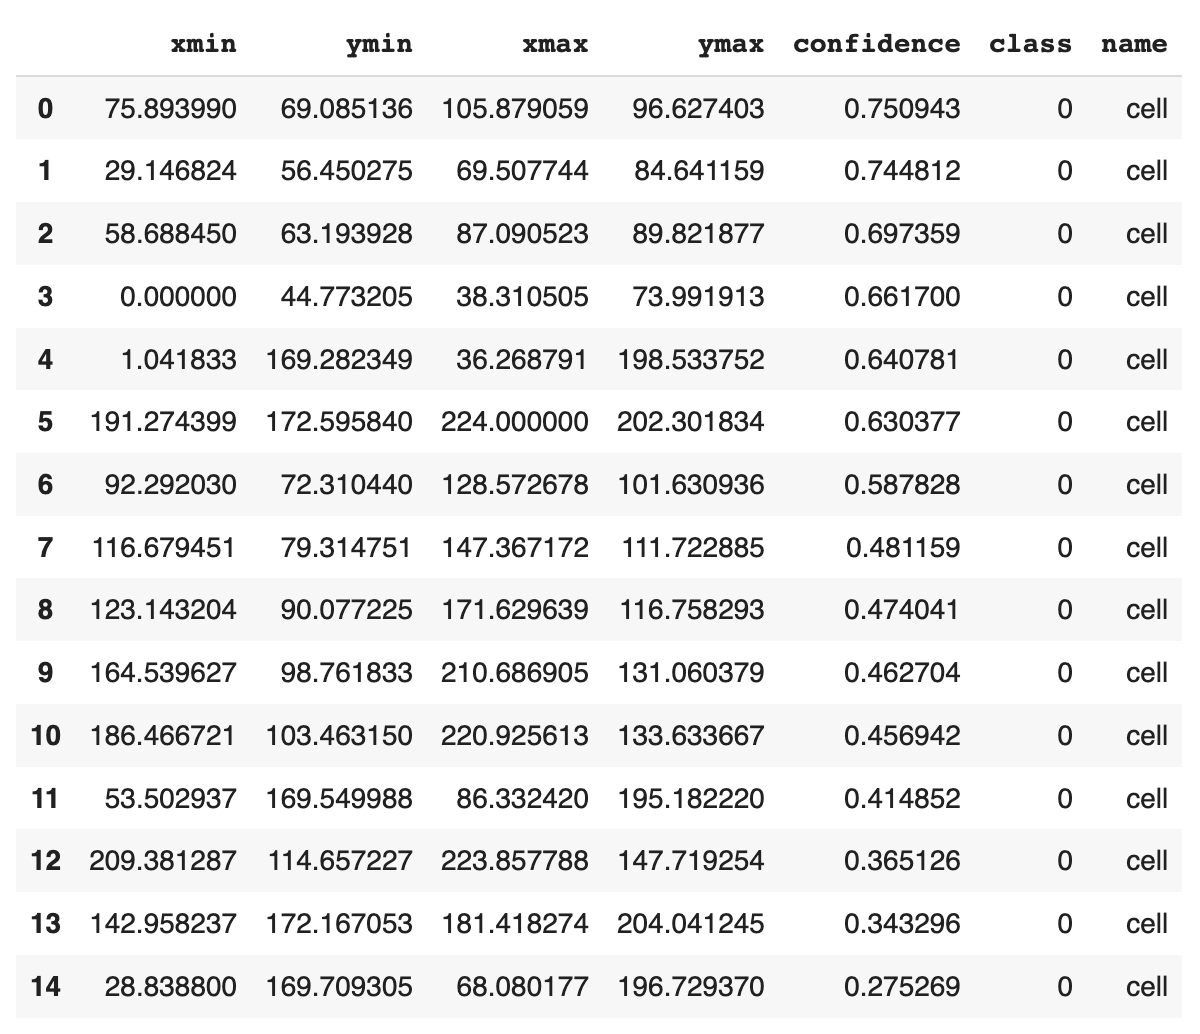
\includegraphics[width=0.8\textwidth]{images/04Implementation/dataframe.png}
	\caption{Predictions by custom YOLOv5 model on a patch from the test set (DataFrame)}
    \label{dataframe}
\end{figure}

\section{Artefact Structure}
A Colab notebook was used to structure the cell counting artefact. This was split into sections and annotated using Markdown to organise all the artefact's components:

\begin{description}
    \item['Preliminaries'] mounts Google Drive, installs and logs into Weights and Biases, and clones YOLOv5 before installing its dependencies.
    
    \item['Training'] simply runs YOLO's \verb|train.py| with the appropriate arguments for \verb|--data|, \verb|--weights|, and other hyperparameters, producing a model.
    
    \item['Counting'] loads a previously trained model and runs \verb`count(...)` using it. This is performed on all 4 images in the test set, returning counts for each.
    
    \item['Evaluation'] computes the model's numerical and percentage error rates for each image, and returns them in a Pandas DataFrame and a LaTeX-format table.
\end{description}